%%%%%%%%%%%%%%%%%%%%%%%%%%%%%%%%%%%%%%%%%
% University Assignment Title Page 
% LaTeX Template
% Version 1.0 (27/12/12)
%
% This template has been downloaded from:
% http://www.LaTeXTemplates.com
%
% Original author:
% WikiBooks (http://en.wikibooks.org/wiki/LaTeX/Title_Creation)
%
% License:
% CC BY-NC-SA 3.0 (http://creativecommons.org/licenses/by-nc-sa/3.0/)
%
%%%%%%%%%%%%%%%%%%%%%%%%%%%%%%%%%%%%%%%%%

%----------------------------------------------------------------------------------------
%	PACKAGES AND OTHER DOCUMENT CONFIGURATIONS
%----------------------------------------------------------------------------------------

\documentclass[12pt]{article}
\usepackage[english]{babel}
\usepackage[utf8x]{inputenc}
\usepackage{amsmath}
\usepackage{graphicx}

\begin{document}

%----------------------------------------------------------------------------------------
%	TITLEPAGE
%----------------------------------------------------------------------------------------

\begin{titlepage}

    \newcommand{\HRule}{\rule{\linewidth}{0.5mm}} % Defines a new command for the horizontal lines, change thickness here

    \center % Center everything on the page

    %----------------------------------------------------------------------------------------
    %	HEADING SECTIONS
    %----------------------------------------------------------------------------------------

    \textsc{\LARGE Università degli studi di Milano-Bicocca}\\[1cm] % Name of your university/college
    \textsc{\Large Advanced Machine Learning }\\[0.3cm] % Major heading such as course name
    \textsc{\large Final Project}\\[0.1cm] % Minor heading such as course title

    %----------------------------------------------------------------------------------------
    %	TITLE SECTION
    %----------------------------------------------------------------------------------------

    \HRule \\[0.4cm]
    { \huge \bfseries Music Genre Classification}\\[0.4cm] % Title of your document
    \HRule \\[1.5cm]

    %----------------------------------------------------------------------------------------
    %	AUTHOR SECTION
    %----------------------------------------------------------------------------------------

    \large
    \emph{Authors:}\\
    Davide Pietrasanta - 844824 - d.pietrasanta@campus.unimib.it  \\   % Your name
    Giuseppe Magazzù - 829612 - g.magazzu1@campus.unimib.it   \\ % Your name
    Gaetano Magazzù - 829685 - g.magazzu2@campus.unimib.it   \\[0.4cm] % Your name

    %----------------------------------------------------------------------------------------
    %	DATE SECTION
    %----------------------------------------------------------------------------------------

    {\large \today}\\[2cm] % Date, change the \today to a set date if you want to be precise

    %----------------------------------------------------------------------------------------
    %	LOGO SECTION
    %----------------------------------------------------------------------------------------

    
\includegraphics{images/logo.png}\\[1cm] % Include a department/university logo - this will require the graphicx package

    %----------------------------------------------------------------------------------------

    \vfill % Fill the rest of the page with whitespace

\end{titlepage}



%----------------------------------------------------------------------------------------
%	ABSTRACT
%----------------------------------------------------------------------------------------

\begin{abstract}
The ABSTRACT is not a part of the body of the report itself. 
Rather, the abstract is a brief summary of the report contents that is often separately circulated so potential readers can decide whether to read the report. 
The abstract should very concisely summarize the whole report: why it was written, what was discovered or developed, and what is claimed to be the significance of the effort. 
The abstract does not include figures or tables, and only the most significant numerical values or results should be given.
\end{abstract}

%----------------------------------------------------------------------------------------
%	SECTIONS
%----------------------------------------------------------------------------------------

\section{Introduction}
The introduction should provide a clear statement of the problem posed by the project, and why the problem is of interest.
It should reflect the scenario, if available.
If needed, the introduction also needs to present background information so that the reader can understand the significance of the problem.
A brief summary of the hypotheses and the approach your group used to solve the problem should be given,
possibly also including a concise introduction to theory or concepts used later to analyze and to discuss the results.

\section{Datasets}
% In this section the available data sets must be presented.
% The term dataset refers to any type of information source, for example web services for geolocation fall into this category.
% In addition, all necessary data manipulation processes, such as cleaning and enrichment with external sources, must be presented and discussed.

The dataset chosen is the Free Music Archive (FMA) \cite{fma_dataset}.
The dataset contains 106574 high quality audio tracks lasting approximately 30 seconds. All the tracks are common creative licensed.

Each track is associated with additional information about the artist (name, location, bio, etc.), the album (title, listens, comments, etc.) and the track itself (title, creation date, duration, genres, etc.).

The genres are organized in a hierarchy of 161 unbalanced classes of different genres.

%Pre-calculated features are also provided: STFT Chromagram, CQT Chromagram, Chroma Energy Normalized (CENS), Tonal Centroid Features (Tonnetz),
%RMSE, Zero Crossing Rate, Spectral Centroid, Spectral Bandwidth, Spectral Contrast, Spectral Rolloff, Mel Frequency Cepstral Coefficients (MFCC). 
%Statistical moments are provided for each of these features: mean, std, skew, kurtosis, median, min, max.
Pre-computed features are also provided such as the statistical moments of some spectral and temporal features.

The dataset propose a train/validation/test (80\%/10\%/10\%) split and three subsets (small, medium, large).
In this work only the small one was used which consists of 8000 tracks and 8 balanced genres.
% \begin{itemize}
%   \item Small: 8000 tracks, 8 balanced genres 
%   \item Medium: 25000 tracks, 16 unbalanced genres
%   \item Large: 106574 tracks, 161 unbalanced genres
% \end{itemize}

\subsection{Preprocessing for CNN}
To use CNN, it was decided to use image spectrograms as input.
Since the dataset did not provide these features, a brief exploratory data analysis was performed.

Analyzing the raw audio tracks it was found that the sampling frequency varies between 22050Hz and 48000Hz.
Most of the tracks have a sampling rate of 44100Hz.
It was decided to resample all tracks to 22050Hz.

Furthermore, it was found that the durations of the audio tracks are not all 30 seconds long.
The range of duration values that was found was from 0 to 30.02 seconds.
Then the length was reduced for all tracks to 29.70 seconds and the shorter length samples were removed due to incorrect length metadata\footnotemark{}.


The logarithmic Mel spectrogram was calculated on the raw audio with the following parameters:
\begin{itemize}
  \item Sample rate: 22050Hz
  \item Window Size: 2048
  \item Hop Length: 512
  \item Mel bins: 128
\end{itemize}

\subsection{Data Augmentation}
Two new spectrograms were generated from each image of the training split using frequency masking and time masking techniques.

Masking consists of setting a range of pixels to zero in the frequency range or time range.

The pixel range is randomly generated from a uniform distribution. For the frequency (0, 27) was used, while for the time (0, 100) \cite{park2019specaugment}.

\footnotetext{more details: \href{https://github.com/mdeff/fma/wiki\#excerpts-shorter-than-30s-and-erroneous-audio-length-metadata}{excerpts-shorter-than-30s-and-erroneous-audio-length-metadata}}
\newpage

\section{The Methodological Approach}

This is the central and most important section of the report.
Its objective must be to show, with linearity and clarity, the steps that have led to the definition of a decision model.
The description of the working hypotheses, confirmed or denied, can be found in this section together with the description of the subsequent refining processes of the models.
Comparisons between different models (e.g. heuristics vs. optimal models) in terms of quality of solutions, their explainability and execution times are welcome.

Do not attempt to describe all the code in the system, and do not include large pieces of code in this section, use pseudo-code where necessary.
Complete source code should be provided separately (in Appendixes, as separated material or as a link to an on-line repo).
Instead pick out and describe just the pieces of code which, for example:
\begin{itemize}
    \item are especially critical to the operation of the system;
    \item you feel might be of particular interest to the reader for some reason;
    \item illustrate a non-standard or innovative way of implementing an algorithm, data structure, etc..
\end{itemize}

You should also mention any unforeseen problems you encountered when implementing the
system and how and to what extent you overcame them. Common problems are:
difficulties involving existing software.

\section{Results and Evaluation}
The following results were obtained with the following hardware.

\vspace{4mm}
\noindent
\begin{minipage}{0.45\textwidth}
  CPU Specifications:
  \begin{itemize}
    \item Intel(R) Xeon(R)
    \item CPU Freq. of 2.30GHz
    \item 4 CPU cores
    \item 16 Gigabytes of RAM
  \end{itemize}
\end{minipage}
\hfill
\begin{minipage}{0.5\textwidth}
  GPU Specifications:
  \begin{itemize}
    \item Nvidia P100
    \item GPU Memory Clock of 1.32GHz
    \item 2 CPU cores
    \item 12 Gigabytes of RAM
  \end{itemize}
\end{minipage}
\vspace{4mm}

\subsection{Handcrafted Features}
\begin{table}[ht]
  \centering
  \begin{tabular}{|l|l|l|l|l|}
    \hline
    \textbf{Units} & \textbf{Parameters} & \textbf{Train Loss} & \textbf{Val Loss} & \textbf{Test Loss} \\ \hline
    (512, 512)     & 532,488             & 1.482               & 1.723             & 1.898              \\ \hline
    (512, 256)     & 399,112             & 1.470               & 1.715             & 1.900              \\ \hline
    (256, 256)     & 200,712             & 1.503               & 1.733             & 1.946              \\ \hline
    (256, 64)      & 149,832             & 1.475               & 1.733             & 1.943              \\ \hline
    (128, 64)      & 75,208              & 1.476               & 1.729             & 1.905              \\ \hline
    (64)           & 33,736              & 1.332               & 1.598             & 1.790              \\ \hline
    (128)          & 67,464              & 1.321               & 1.577             & 1.800              \\ \hline
    (256)          & 134,920             & 1.338               & 1.592             & 1.806              \\ \hline
    (512)          & 269,832             & 1.334               & 1.579             & 1.803              \\ \hline
  \end{tabular}
  \caption{Values of loss for the different number of neurons.}
  \label{table:handcrafted_loss}
\end{table}

\begin{table}[ht]
  \centering
  \begin{tabular}{|l|l|l|l|l|}
    \hline
    \textbf{Units} & \textbf{Parameters} & \textbf{Train Acc} & \textbf{Val Acc} & \textbf{Test Acc} \\ \hline
    (512, 512)     & 532,488             & 0.677              & 0.563            & 0.487             \\ \hline
    (512, 256)     & 399,112             & 0.680              & 0.567            & \textbf{0.495}    \\ \hline
    (256, 256)     & 200,712             & 0.683              & 0.577            & 0.482             \\ \hline
    (256, 64)      & 149,832             & 0.690              & 0.577            & 0.484             \\ \hline
    (128, 64)      & 75,208              & 0.683              & 0.564            & 0.489             \\ \hline
    (64)           & 33,736              & 0.680              & 0.560            & 0.465             \\ \hline
    (128)          & 67,464              & 0.686              & 0.566            & 0.475             \\ \hline
    (256)          & 134,920             & 0.685              & 0.566            & 0.479             \\ \hline
    (512)          & 269,832             & 0.683              & 0.571            & 0.472             \\ \hline
  \end{tabular}
  \caption{Values of accuracy for the different number of neurons.}
  \label{table:handcrafted_accuracy}
\end{table}

\newpage

\begin{figure}
  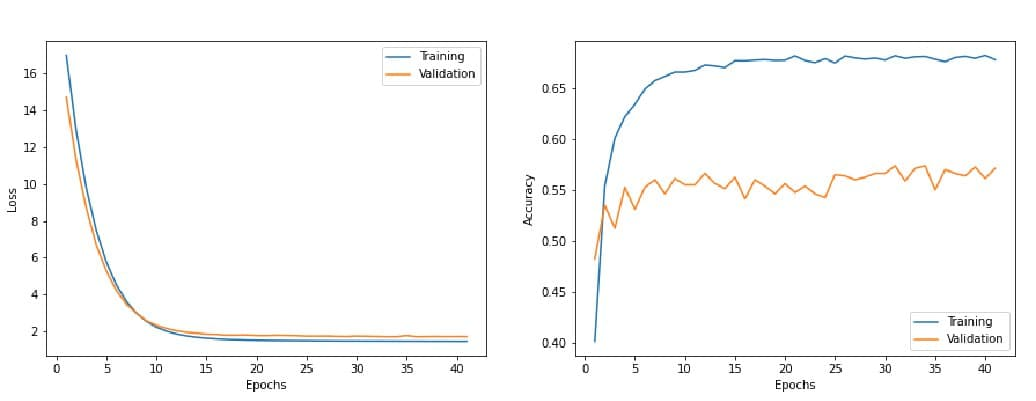
\includegraphics[width=\textwidth]{images/handcrafted_best.jpg}
  \caption{Loss and Accuracy curves for the best model.}
\end{figure}

\pagebreak

\subsection{CNN}
The following tables compare CNN with and without augmentation and with and without tuning in terms of prediction time, accuracy and loss.

\begin{table}[ht]
  \begin{tabular}{|l|l|l|l|}
    \hline
                        & Prediction time (CPU) & Prediction time (GPU) \\ \hline
    CNN                 & 0.064s                & 0.042s                \\ \hline
    Tuned CNN           & 0.060s                & 0.043s                \\ \hline
    Tuned CNN augmented & 0.061s                & 0.044s                \\ \hline
  \end{tabular}
  \caption{Inference time over 10 runs of the same random value for CNN models.}
  \label{table:pred_time}
\end{table}

\begin{table}[ht]
  \centering
  \begin{tabular}{|l|l|l|l|}
    \hline
                        & Test accuracy   & Test Loss \\ \hline
    CNN                 & \textbf{0.3975} & 3.7596    \\ \hline
    CNN augmented       & 0.3225          & 8.0137    \\ \hline
    Tuned CNN           & 0.3900          & 2.3860    \\ \hline
    Tuned CNN augmented & 0.3787          & 2.0166    \\ \hline
  \end{tabular}
  \caption{Test accuracy and loss of the CNN models.}
  \label{table:test_CNN}
\end{table}

\newpage

\begin{table}[ht]
  \centering
  \begin{tabular}{|l|l|l|}
    \hline
                        & Train accuracy & Train Loss \\ \hline
    CNN                 & 0.9998         & 0.0011     \\ \hline
    CNN augmented       & 0.9968         & 0.0101     \\ \hline
    Tuned CNN           & 0.9998         & 0.0065     \\ \hline
    Tuned CNN augmented & 0.8073         & 0.6131     \\ \hline
  \end{tabular}
  \caption{Train accuracy and loss of the CNN models.}
  \label{table:train_CNN}
\end{table}

\begin{table}[ht]
  \centering
  \begin{tabular}{|l|l|l|}
    \hline
                        & Validation accuracy & Validation Loss \\ \hline
    CNN                 & 0.4663              & 2.9336          \\ \hline
    CNN augmented       & 0.3938              & 5.6310          \\ \hline
    Tuned CNN           & 0.4175              & 2.0767          \\ \hline
    Tuned CNN augmented & 0.4450              & 1.7493          \\ \hline
  \end{tabular}
  \caption{Validation accuracy and loss of the CNN models.}
  \label{table:validation_CNN}
\end{table}

\newpage

\begin{figure}[ht]
  \centering
  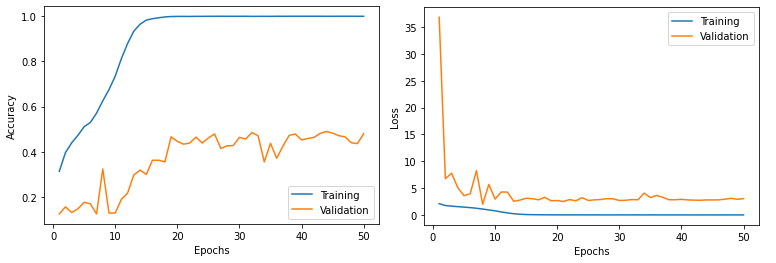
\includegraphics[scale=0.6]{images/2021-val-train.png}
  \caption{CNN's Accuracy and Loss function of the training and validation set.}
  \label{fig:Acc_Loss_2021}
\end{figure}

\begin{figure}[ht]
  \centering
  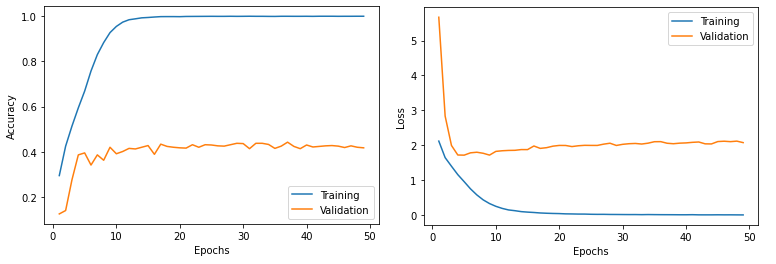
\includegraphics[scale=0.6]{images/tuned-val-train.png}
  \caption{Tuned CNN's Accuracy and Loss function of the training and validation set.}
  \label{fig:Acc_Loss_tuned}
\end{figure}

\newpage

\begin{figure}[ht]
  \centering
  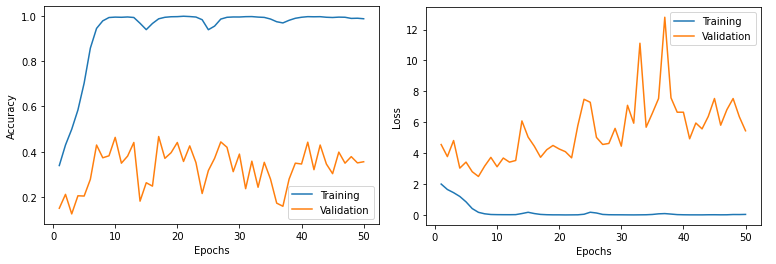
\includegraphics[scale=0.6]{images/aug-2021-val-train.png}
  \caption{CNN's Accuracy and Loss function of the training and validation set with data augmentation.}
  \label{fig:Acc_Loss_2021_aug}
\end{figure}

\begin{figure}[ht]
  \centering
  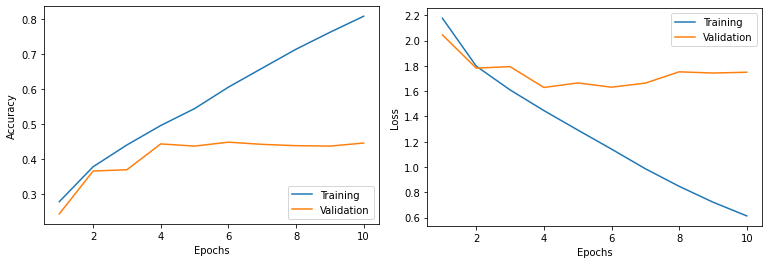
\includegraphics[scale=0.6]{images/aug-tuned-val-train.png}
  \caption{Tuned CNN's Accuracy and Loss function of the training and validation set with data augmentation.}
  \label{fig:Acc_Loss_tuned_aug}
\end{figure}

\newpage

\begin{figure}[ht]
  \begin{subfigure}[c]{0.475\textwidth}
    \centering
    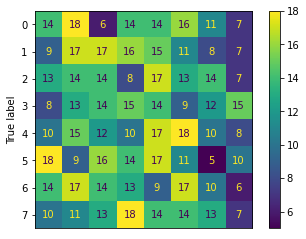
\includegraphics[width=\textwidth]{images/2021-confusion_matrix.png}
    \caption{Simple CNN}
    \label{fig:cf_2021}
  \end{subfigure}
  \hfill
  \begin{subfigure}[c]{0.475\textwidth}
    \centering
    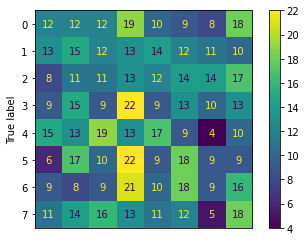
\includegraphics[width=\textwidth]{images/tuned-confusion_matrix.png}
    \caption{Tuned CNN}
    \label{fig:cf_tuned}
  \end{subfigure}
  \caption{CNN's confusion matrix.}
\end{figure}


\begin{figure}[ht]
  \begin{subfigure}[c]{0.475\textwidth}
    \centering
    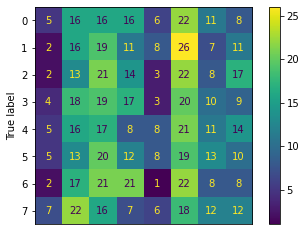
\includegraphics[width=\textwidth]{images/aug-2021-confusion_matrix.png}
    \caption{Simple CNN}
    \label{fig:cf_2021_aug}
  \end{subfigure}
  \hfill
  \begin{subfigure}[c]{0.475\textwidth}
    \centering
    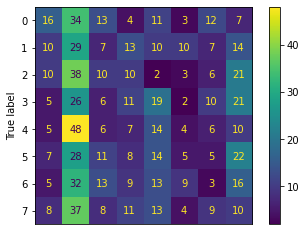
\includegraphics[width=\textwidth]{images/aug-tuned-confusion_matrix.png}
    \caption{Tuned CNN}
    \label{fig:cf_tuned_aug}
  \end{subfigure}
  \caption{CNN's confusion matrix with data augmentation.}
\end{figure}

\newpage
\subsection{Feature Extracted with CNN}

\begin{table}[ht]
  \centering
  \resizebox{\textwidth}{!}{%
    \begin{tabular}{|c|c|c|c|c|ccc|}
      \hline
      \multirow{2}{*}{Cut Level} & \multirow{2}{*}{Size} & \multirow{2}{*}{Size after PCA} & \multirow{2}{*}{PCA value} & \multirow{2}{*}{Model} & \multicolumn{3}{c|}{Accuracy}                                                           \\ \cline{6-8}
                                 &                       &                                 &                            &                        & \multicolumn{1}{c|}{svm linear}    & \multicolumn{1}{c|}{svm rbf}       & mlp           \\ \hline
      Fc2                        & 4096                  & 1480                            & 0.99                       & VGG16                  & \multicolumn{1}{c|}{0.4440/0.4003} & \multicolumn{1}{c|}{0.5168/0.4454} & 0.4795/0.4191 \\ \hline
      Fc2                        & 4096                  & 429                             & 0.95                       & VGG16                  & \multicolumn{1}{c|}{0.4965/0.4530} & \multicolumn{1}{c|}{0.5206/0.4542} & 0.4890/0.4361 \\ \hline
      Fc2                        & 4096                  & 153                             & 0.9                        & VGG16                  & \multicolumn{1}{c|}{0.5099/0.4586} & \multicolumn{1}{c|}{0.5195/0.4617} & 0.4920/0.4398 \\ \hline
    \end{tabular}%
  }
  \caption{Results of the FC2 cut level of VGG16 with different classifier and different values of PCA.}  \label{tab:my-table}
\end{table}

\begin{table}[ht]
  \centering
  \resizebox{\textwidth}{!}{%
    \begin{tabular}{|c|c|c|c|}
      \hline
      N             & svm linear    & svm rbf                      & mlp                                                   \\ \hline
      FC2, PCA 0.99 & \{'C': 0.01\} & \{'C': 10, 'gamma': 0.0001\} & \{'alpha': 0.03, 'hidden\_layer\_sizes': (512, 32)\}  \\ \hline
      FC2, PCA 0.95 & \{'C': 0.01\} & \{'C': 10, 'gamma': 0.0001\} & \{'alpha': 0.05, 'hidden\_layer\_sizes': (512, 32)\}  \\ \hline
      FC2, PCA 0.90 & \{'C': 0.01\} & \{'C': 10, 'gamma': 0.0001\} & \{'alpha': 0.05, 'hidden\_layer\_sizes': (512, 256)\} \\ \hline
    \end{tabular}%
  }
  \caption{Hyperparameters results for the VGG16 FC2 with different values of pca.}
  \label{tab:my-table}
\end{table}

\begin{table}[ht]
  \centering
  \resizebox{\textwidth}{!}{%
    \begin{tabular}{|c|c|c|c|ccc|}
      \hline
      \multirow{2}{*}{Cut Level} & \multirow{2}{*}{Size} & \multirow{2}{*}{Size after PCA} & \multirow{2}{*}{Model} & \multicolumn{3}{c|}{Accuracy}                                                                     \\ \cline{5-7}
                                 &                       &                                 &                        & \multicolumn{1}{c|}{svm linear}    & \multicolumn{1}{c|}{svm rbf}                 & mlp           \\ \hline
      Fc2                        & 4096                  & 153                             & VGG16                  & \multicolumn{1}{c|}{0.5099/0.4586} & \multicolumn{1}{c|}{0.5195/0.4617}           & 0.4920/0.4398 \\ \hline
      Fc1                        & 4096                  & 311                             & VGG16                  & \multicolumn{1}{c|}{0.5157/0.4573} & \multicolumn{1}{c|}{0.5315/0.4837}           & 0.5076/0.4718 \\ \hline
      block5\_pool               & 7x7x512               & 1174                            & VGG16                  & \multicolumn{1}{c|}{0.4316/0.4185} & \multicolumn{1}{c|}{\textbf{0.5317/ 0.4968}} & 0.4726/0.4429 \\ \hline
    \end{tabular}%
  }
  \caption{Results of different cut levels with PCA 90\% on the VGG16 with classical classifiers.}
  \label{tab:my-table2}
\end{table}

\begin{table}[ht]
  \centering
  \resizebox{\textwidth}{!}{%
    \begin{tabular}{|c|c|c|c|}
      \hline
      Cut Level    & svm linear    & svm rbf                      & mlp                                                   \\ \hline
      Fc2          & \{'C': 0.01\} & \{'C': 10, 'gamma': 0.0001\} & \{'alpha': 0.05, 'hidden\_layer\_sizes': (512, 256)\} \\ \hline
      Fc1          & \{'C': 0.01\} & \{'C': 10, 'gamma': 0.0001\} & \{'alpha': 0.05, 'hidden\_layer\_sizes': (512, 32)\}  \\ \hline
      block5\_pool & \{'C': 0.01\} & \{'C': 1, 'gamma': 0.0001\}  & \{'alpha': 0.03, 'hidden\_layer\_sizes': (512, 256)\} \\ \hline
    \end{tabular}%
  }
  \caption{Hyperparameters result for different cut level of VGG16 with PCA 90\%.}
  \label{tab:my-table}
\end{table}

\begin{table}[ht]
  \centering
  \resizebox{\textwidth}{!}{%
    \begin{tabular}{|c|c|c|c|ccc|}
      \hline
      \multirow{2}{*}{Cut Level} & \multirow{2}{*}{Size} & \multirow{2}{*}{Size after PCA} & \multirow{2}{*}{Model} & \multicolumn{3}{c|}{Accuracy}                                                                    \\ \cline{5-7}
                                 &                       &                                 &                        & \multicolumn{1}{c|}{svm linear}    & \multicolumn{1}{c|}{svm rbf}                & mlp           \\ \hline
      avg\_pool                  & 1000                  & 87                              & ResNet50               & \multicolumn{1}{c|}{0.5268/0.4649} & \multicolumn{1}{c|}{0.5381/0.4874}          & 0.5246/0.4592 \\ \hline
      conv5\_block1\_2\_relu     & 7x7x512               & 1321                            & ResNet50               & \multicolumn{1}{c|}{0.4193/0.4104} & \multicolumn{1}{c|}{\textbf{0.5484/0.5012}} & 0.5221/0.4755 \\ \hline
    \end{tabular}%
  }
  \caption{Results of different cut levels with PCA 90\% on the ResNet50 with classical classifiers.}
  \label{tab:my-table3}
\end{table}

\newpage

\begin{table}[ht]
  \centering
  \resizebox{\textwidth}{!}{%
    \begin{tabular}{|c|c|c|c|}
      \hline
      Cut Level              & svm linear    & svm rbf                      & mlp                                                  \\ \hline
      avg\_pool              & \{'C': 0.01\} & \{'C': 10, 'gamma': 0.0001\} & \{'alpha': 0.05, 'hidden\_layer\_sizes': (512, 32)\} \\ \hline
      conv5\_block1\_2\_relu & \{'C': 0.01\} & \{'C': 10, 'gamma': 0.0001\} & \{'alpha': 0.01, 'hidden\_layer\_sizes': (512,)\}    \\ \hline
    \end{tabular}%
  }
  \caption{Hyperparameters result for different cut of ResNet50 with PCA 90\%.}
  \label{tab:my-table}
\end{table}

\begin{figure}[ht]
  \begin{subfigure}[c]{0.475\textwidth}
    \centering
    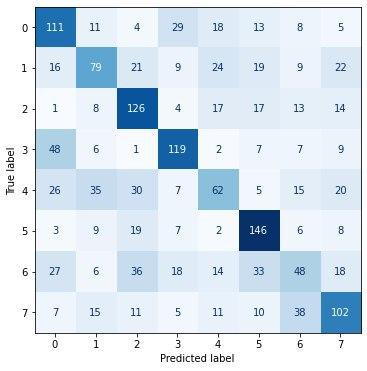
\includegraphics[width=\textwidth]{images/best_vgg16_svmrbf.jpg}
    \caption{VGG16 - SVM RBF}
    \label{fig:best_vgg16_svmrbf_cm}
  \end{subfigure}
  \hfill
  \begin{subfigure}[c]{0.475\textwidth}
    \centering
    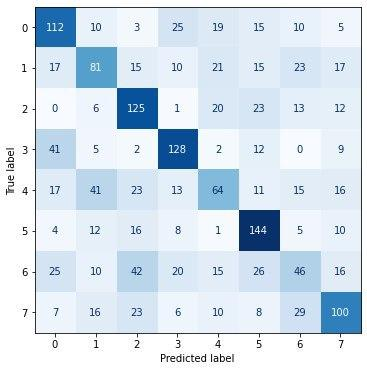
\includegraphics[width=\textwidth]{images/best_resnet50_svmrbf.jpg}
    \caption{ResNet50 - SVM RBF}
    \label{fig:best_resnet50_svmrbf_cm}
  \end{subfigure}
  \caption{Confusion matrix of the best model for the two CNN architectures.}
\end{figure}

\begin{table}[ht]
  \centering
  \resizebox{\textwidth}{!}{%
    \begin{tabular}{|c|c|c|c|}
      \hline
      Model          & Test Time(CPU) & Test Time(GPU) & svm rbf   \\ \hline
      vgg16\_best    & 73.2190 ms     & 23.9014 ms     & 2.6992 ms \\ \hline
      resnet50\_best & 51.3436 ms     & 23.7502 ms     & 3.2712 ms \\ \hline
    \end{tabular}%
  }
  \caption{inference time for the best cut level and ml classifier for vgg16 and resnet50.}
  \label{tab:my-table4}
\end{table}

\newpage

\section{Discussion}
The discussion section aims at interpreting the results in light of the project's objectives.
The most important goal of this section is to interpret the results so that the reader is informed of the insight or answers that the results provide.
This section should also present an evaluation of the particular approach taken by the group.
For example: Based on the results, how could the experimental procedure be improved?
What additional, future work may be warranted?
What recommendations can be drawn?


\begin{figure}[ht]
\centering
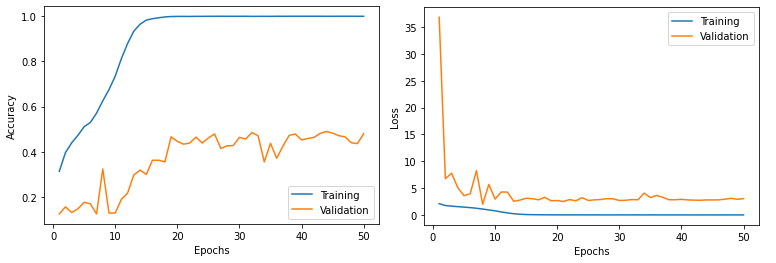
\includegraphics[scale=0.6]{images/2021-val-train.png}
\caption{Accuracy and Loss function of the training and validation set.}
\label{fig:GP_Acq}
\end{figure}


\begin{figure}[ht]
\centering
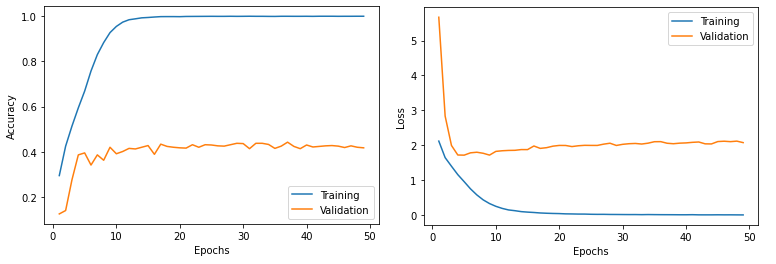
\includegraphics[scale=0.6]{images/tuned-val-train.png}
\caption{Accuracy and Loss function of the training and validation set.}
\label{fig:GP_Acq}
\end{figure}

\section{Conclusions}

Various methods for classifying audio genres have been tried.
The approach based on spectrograms and Convolutional Neural Networks was the worst. 
The Handcrafted Features based approach proved to be a good alternative. 
The approach with the best results turned out to be the one based on Transfer Learning.
The use of spectrograms is however indispensable for these types of problems.


%----------------------------------------------------------------------------------------
%	BIBLIOGRAPHY
%----------------------------------------------------------------------------------------

\section*{References}

The references section should contain complete citations following standard form.  
The references should be numbered and listed in the order they were cited in the body of the report. 
In the text of the report, a particular reference can be cited by using a numerical number in brackets as \cite{kostrzewa2021music} that corresponds to its number in the reference list. 
\LaTeX provides several styles to format the references

\bibliographystyle{IEEEtran}
\bibliography{references.bib}

\end{document}